
\documentclass[]{article}

\usepackage{graphicx}
\usepackage[margin=1.5cm,top=1.5cm,bottom=1.5cm,a4paper]{geometry}
\usepackage{graphicx} % Required for inserting images
\usepackage{titlesec} % Required for customizing section titles
\usepackage[margin=1.5cm,top=1.5cm, bottom=1.5cm]{geometry} % Ajusta los márgenes aquí
\usepackage{multicol} % Required for multicols environment
\usepackage{parskip}
\usepackage{etoolbox}
\usepackage{tcolorbox}
\usepackage{float}
\usepackage{amsmath}
\usepackage{dingbat}
\usepackage{booktabs} 
\usepackage{caption}
\usepackage[utf8]{inputenc}
\usepackage[T1]{fontenc}
\usepackage{amssymb}
\usepackage[spanish]{babel}
\usepackage{multirow}
\usepackage{siunitx}
\usepackage{circuitikz}
\usepackage{pdflscape}
\usepackage{subcaption}
\usepackage{array}
\usepackage{tcolorbox}
\usepackage{xcolor}
\usepackage{pdfpages}
\usepackage{placeins}



\newif\ifcheckpoint
\checkpointfalse

% función que devuelve color según checkpoint
\newcommand{\checkpointcolor}[1]{%
	\ifcase#1
	yellow%
	\or blue%
	\or green%
	\or red%
	\or orange%
	\else gray%
	\fi
}
\newcommand{\checkpointstart}[1]{%
	\ifcheckpoint
	\edef\tempcolor{\checkpointcolor{#1}}%
	\begin{tcolorbox}[
		colback=\tempcolor!15,
		colframe=\tempcolor!60!black,
		boxrule=0pt,
		arc=0pt,
		width=\textwidth
		]
		\textbf{Inicio checkpoint #1}
	\end{tcolorbox}
	\fi
}

\newcommand{\checkpointend}[1]{%
	\ifcheckpoint
	\edef\tempcolor{\checkpointcolor{#1}}%
	\begin{tcolorbox}[
		colback=\tempcolor!15,
		colframe=\tempcolor!60!black,
		boxrule=0pt,
		arc=0pt,
		width=\textwidth
		]
		\textbf{Fin checkpoint #1}
	\end{tcolorbox}
	\fi
}

\usepackage{tikz}
\usetikzlibrary{arrows.meta, positioning}
\usetikzlibrary{babel}

\usepackage{csquotes}

\usepackage[
backend=biber,
style=apa,
citestyle=apa
]{biblatex}

\addbibresource{referencias.bib}


\begin{document}
	
	\begin{titlepage}
		
		\centering
		{
\includegraphics[scale=0.5]{img/Caratula.jpg}}
		
		\centerline
		
		{\bfseries\LARGE Taller de Diseño de Circuitos Electrónicos   \par}
		
		{\bfseries\LARGE TA138  \par}
		\vspace{.5cm}
		{\scshape\Large Facultad de Ingenier\'ia Universidad de Buenos Aires \par}
		\vspace{1.5cm}
		%{\scshape\Huge Trabajo Pr\'actico \par}
		{\scshape\Huge Diseño de Fuente de Alimentación \par}
		\vspace{2cm}
		{\scshape\Large Checkpoint 5: Conversor \textit{Buck}\par}
		
		
		\vspace{2cm}
		
		\begin{tabular}{ p{4cm} p{2cm} p{4cm}}
			\textbf{Alumnos:} & \textbf{Padr\'on:} & \textbf{Mail:} \\
			Lazo, Sebastian Nahuel & 106213 &slazo@fi.uba.ar \\
			Flores, Ahmed Ali & 106238 & aaflores@fi.uba.ar  \\
			Mántaras, Ramiro  & 111510 &rmantaras@fi.uba.ar \\
			
		\end{tabular}
		
		
		\vspace{1cm}
		
		\begin{tabular}{ p{6cm} p{6cm} p{6cm}}
			\textbf{Docentes:}  
			\\Teóricas: Julio Zola & Tutor: Sergio Andres Quinteros  
		\end{tabular}
		
	\end{titlepage}
	
	
	\newpage
	
	
	\tableofcontents \label{Indice}
	\newpage
	\section{Introducción}
	
	En la entrega previa se verifico la fuente \textit{buck} a lazo abierto, se definieron las características físicas del inductor utilizado, se diseño la placa de circuito impreso y se verifico el funcionamiento del modulador de ancho de pulso en la placa.
	

	\section{Objetivo}
		
	\begin{itemize}
		\item 	Caracterización y validación de regulador conmutado en lazo cerrado con implementación de PWM.
		\item 	Diseño de PCB + CEM.
		\item Manual de construcción y validación de producto terminado 	
	\end{itemize}	
		
	
	\section{Desarrollo}
	

	
	\section{Conclusiones}

	
	{\footnotesize
		\printbibliography
	}
	
	
	\newpage
	\appendix

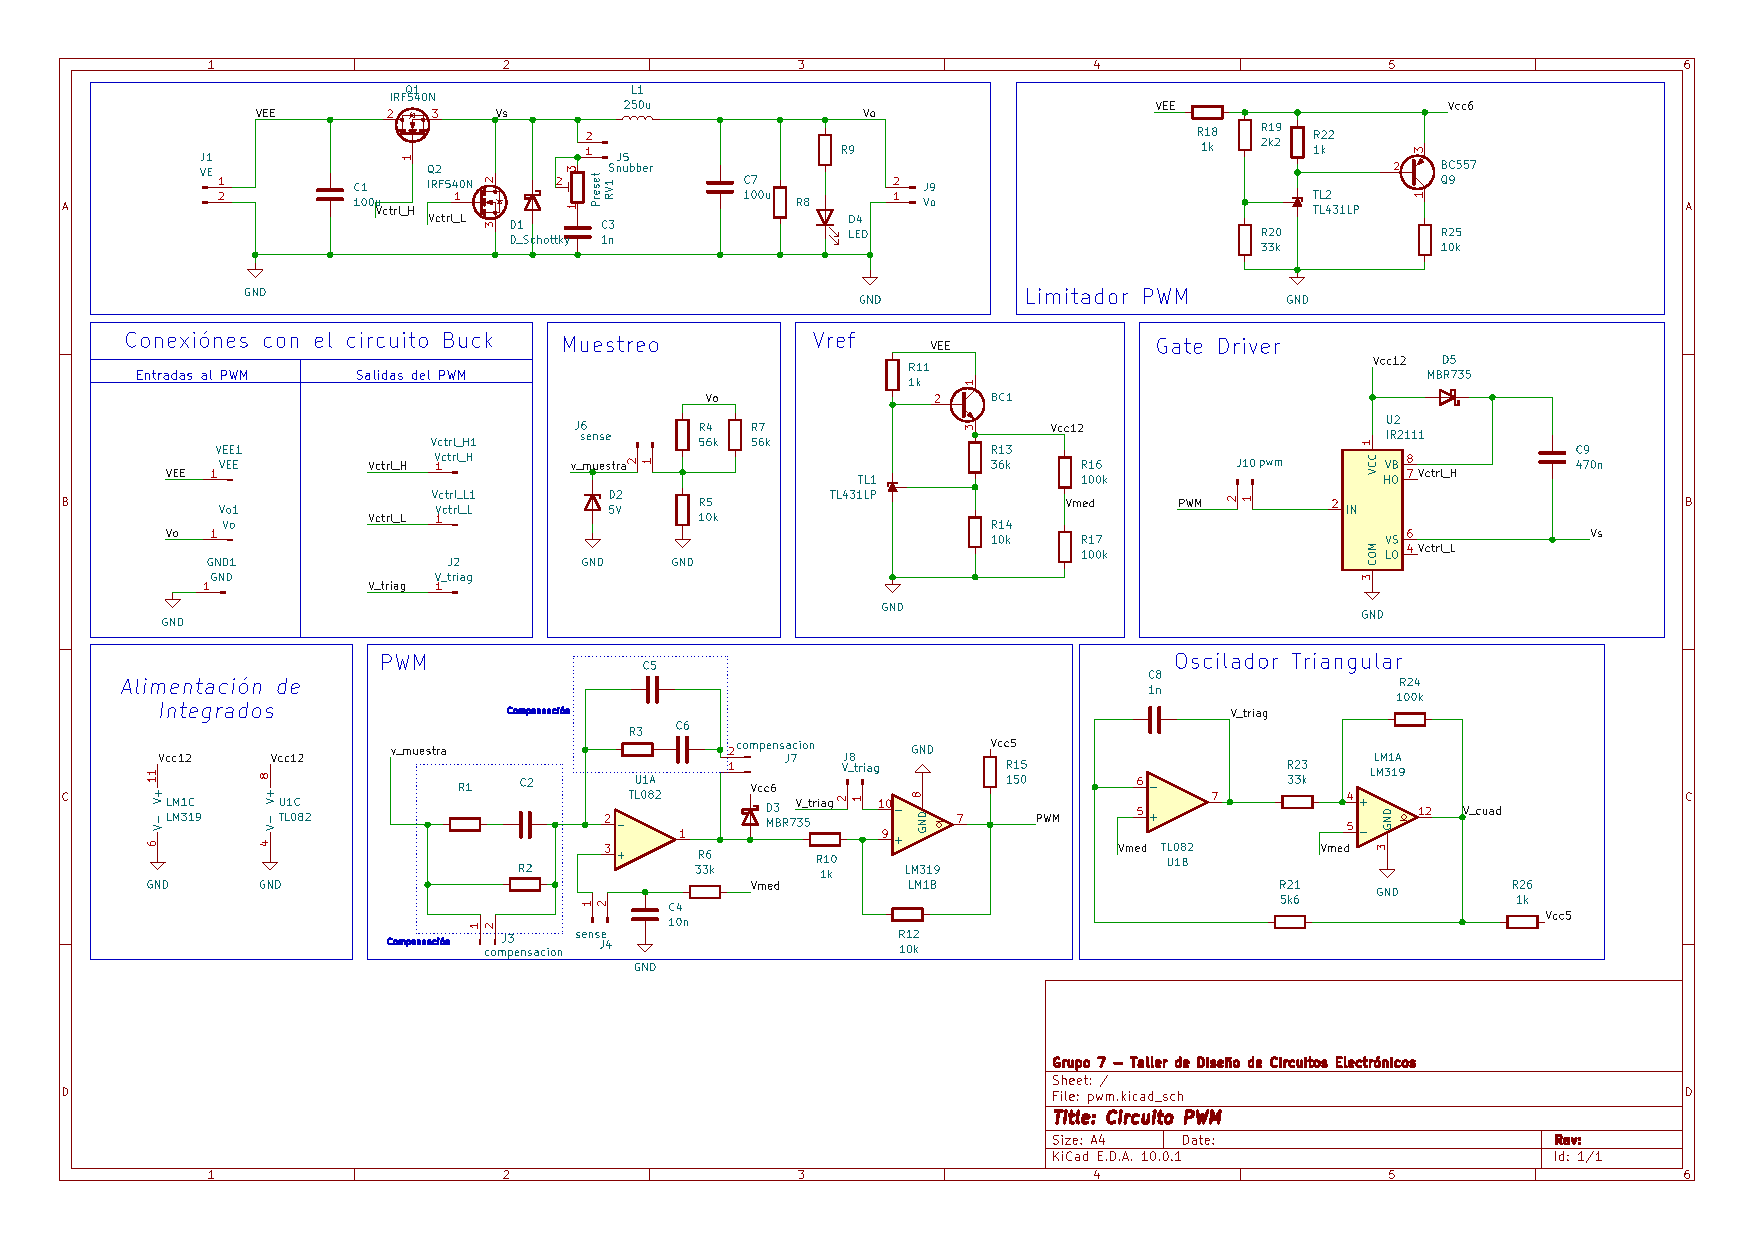
\includepdf[
pages=1,
angle=90,
fitpaper=true,
pagecommand={\section{Apéndice I: PCB}\label{sec:apendice_PCB}\subsection{Esquematico.}}
]{img/BUCK/esquematico_buck.pdf}

\let\clearpage\relax

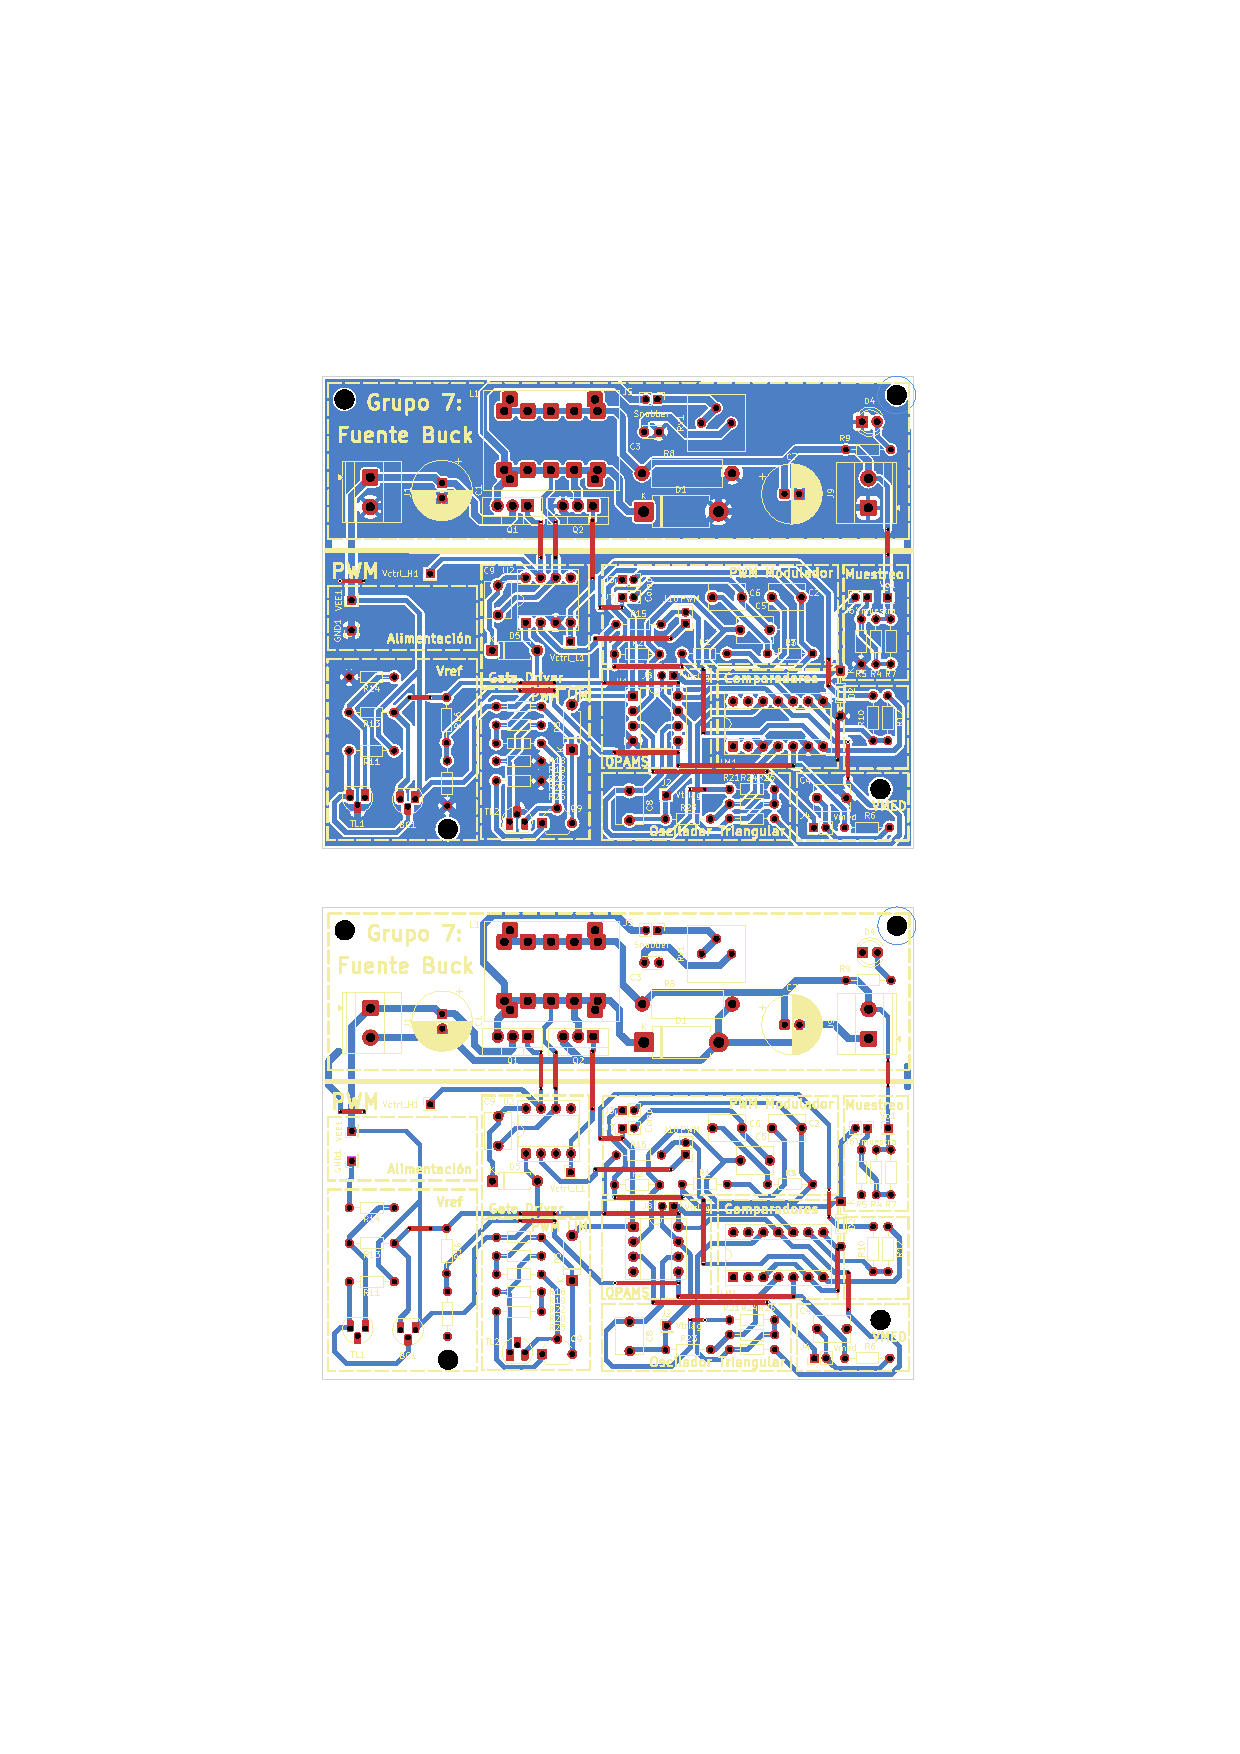
\includepdf[
pages=1,
pagecommand={\subsection{Pistas}}
]{img/BUCK/pistas_buck.pdf}


\end{document}
